\documentclass{article}

\usepackage[czech]{babel}
\usepackage[utf8]{inputenc}
\usepackage[T1]{fontenc}

\usepackage[left=2cm,text={17cm, 24cm},top=3cm, bottom=2cm]{geometry}

\usepackage{rotating}
\usepackage{graphicx} % vkládání obrázků
\usepackage{amsmath} % pokročilá sazba matematiky
% \usepackage{xcolor} % barevný text
% \usepackage[european]{circuitikz} % Obvody
\usepackage{siunitx} % SI jednotky
\usepackage{graphicx} % Obrázky
\usepackage{hyperref} % Clicable table of contents
\usepackage{color} % Color for table of contents
\usepackage{float}
\usepackage{lscape} 

\restylefloat{figure}

\hypersetup{
    colorlinks=true, %set true if you want colored links
    linktoc=all, %set to all if you want both sections and subsections linked
    linkcolor=black,  %choose some color if you want links to stand out
}

\graphicspath{ {./images} } % Include image folder

% \begin{figure}[H] 
%     \centering
%     \includegraphics[scale=0.7,keepaspectratio]{2_2}
%     \caption{Měření VA charakteristiky}
%     \label{fig:va_dioda}
% \end{figure} for icluding image

% important things: \[  \], \tau , \approx , \SI{1}{\micro\farad} , \SI{10}{\kohm}
% \begin{table}[H]
% 	\begin{center}
% 		\begin{tabular}{|c|c|c|c|c|c|c|c|c|c|c|c|c|c|} 
% 			\hline
% 			Ud [V] & 0.00 &  0.20 & 0.40 & 0.60 & 0.80 & 1.00 & 1.20 & 1.40 & 1.60 & 1.71 & 1.78 & 1.80 & 1.81\\
% 			\hline
% 			Id [mA] & 0.00 & 0.00 & 0.00 & 0.00 & 0.00 & 0.00 & 0.00 & 0.00 & 0.09 & 0.25 & 0.42 & 0.60 & 0.79 \\
% 			\hline
% 		\end{tabular}
% 		
% 		\caption{Naměřené hodnoty napětí a proudu diodou}
% 	\end{center}
% \end{table}

\begin{document}

% start first page
\clearpage
\begin{titlepage}
	\begin{center}
		\textsc{\LARGE Vysoké Učení Technické v Brně}\\[0.5cm]
		{\LARGE Fakulta informačních technologií }\\[4.0cm]

		\textsc{\LARGE ISS}\\[0.5cm]
		\textsc{\LARGE 2020/2021}\\[3.5cm]

		{\LARGE Projekt}\\[1.0cm]
	\end{center}

	\vfill 

	\begin{flushleft} 
		\large
		Martin Douša (xdousa00)
		\hfill
		Brno, \today
	\end{flushleft}
\end{titlepage}
\thispagestyle{empty}

\newpage
\tableofcontents

\newpage
\listoffigures

\newpage
% end first page

\section{Základy}
\begin{figure}[H] 
    \centering
    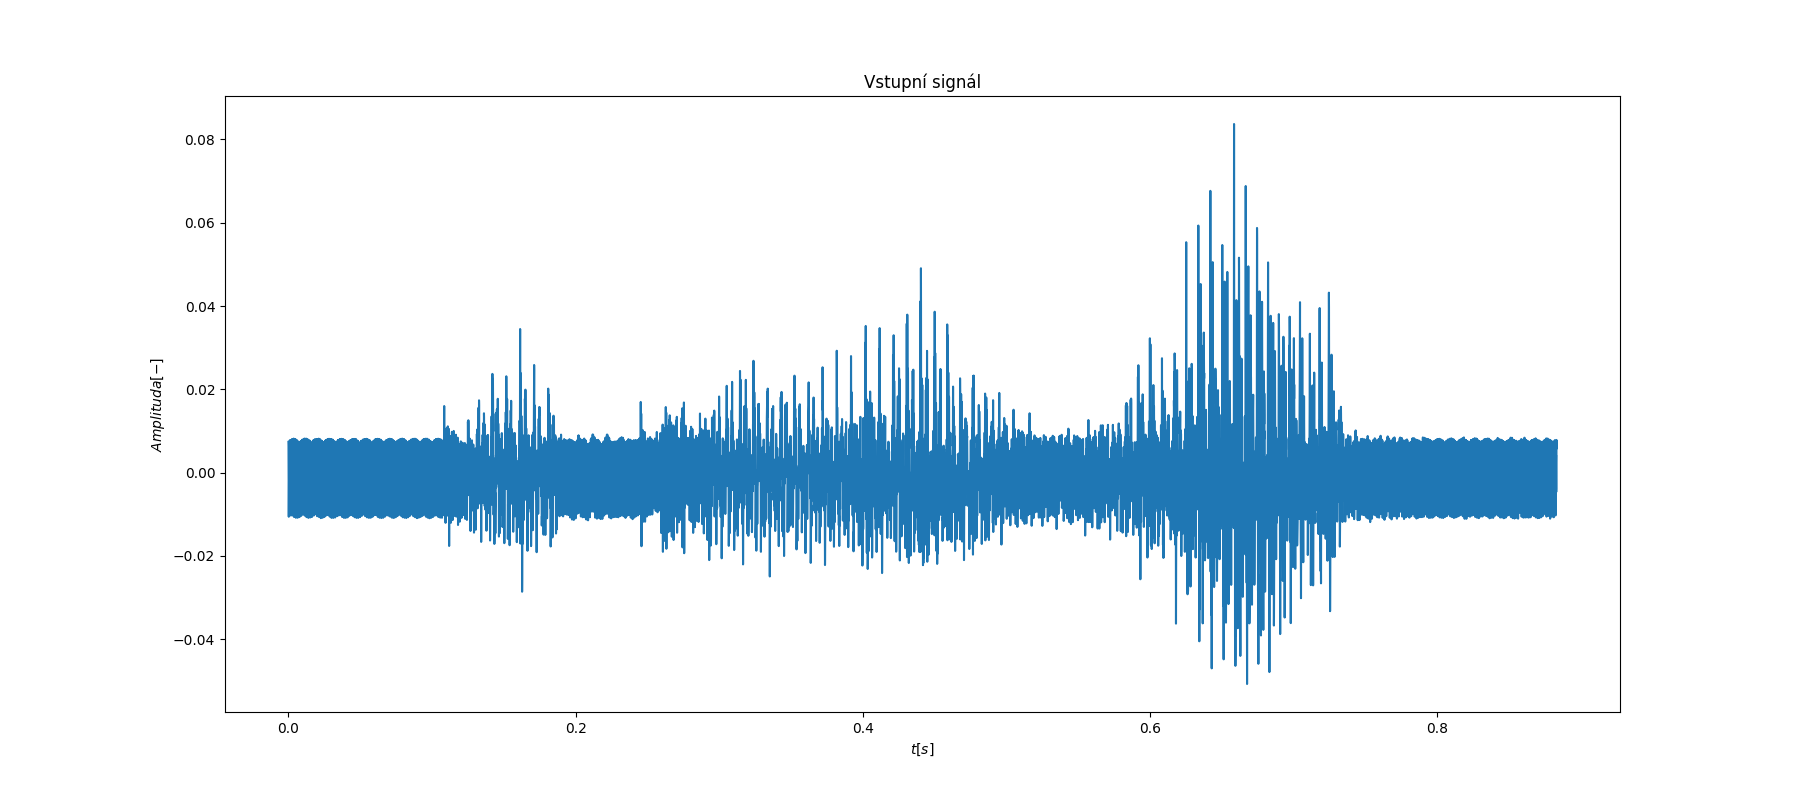
\includegraphics[scale=0.35,keepaspectratio]{Figure_1}
    \caption{Načtený signál}
\end{figure}

Délka vstupního signálu je 14132 vzorků což při vzorkovací frekvenci 16kHz odpovádá 0.88325s.
Maximální hodnota tohoto signálu je přibližně 0.837097 a minimální přibližně -0.050751.

\section{Předzpracování a rámce}
\begin{figure}[H] 
	\centering
	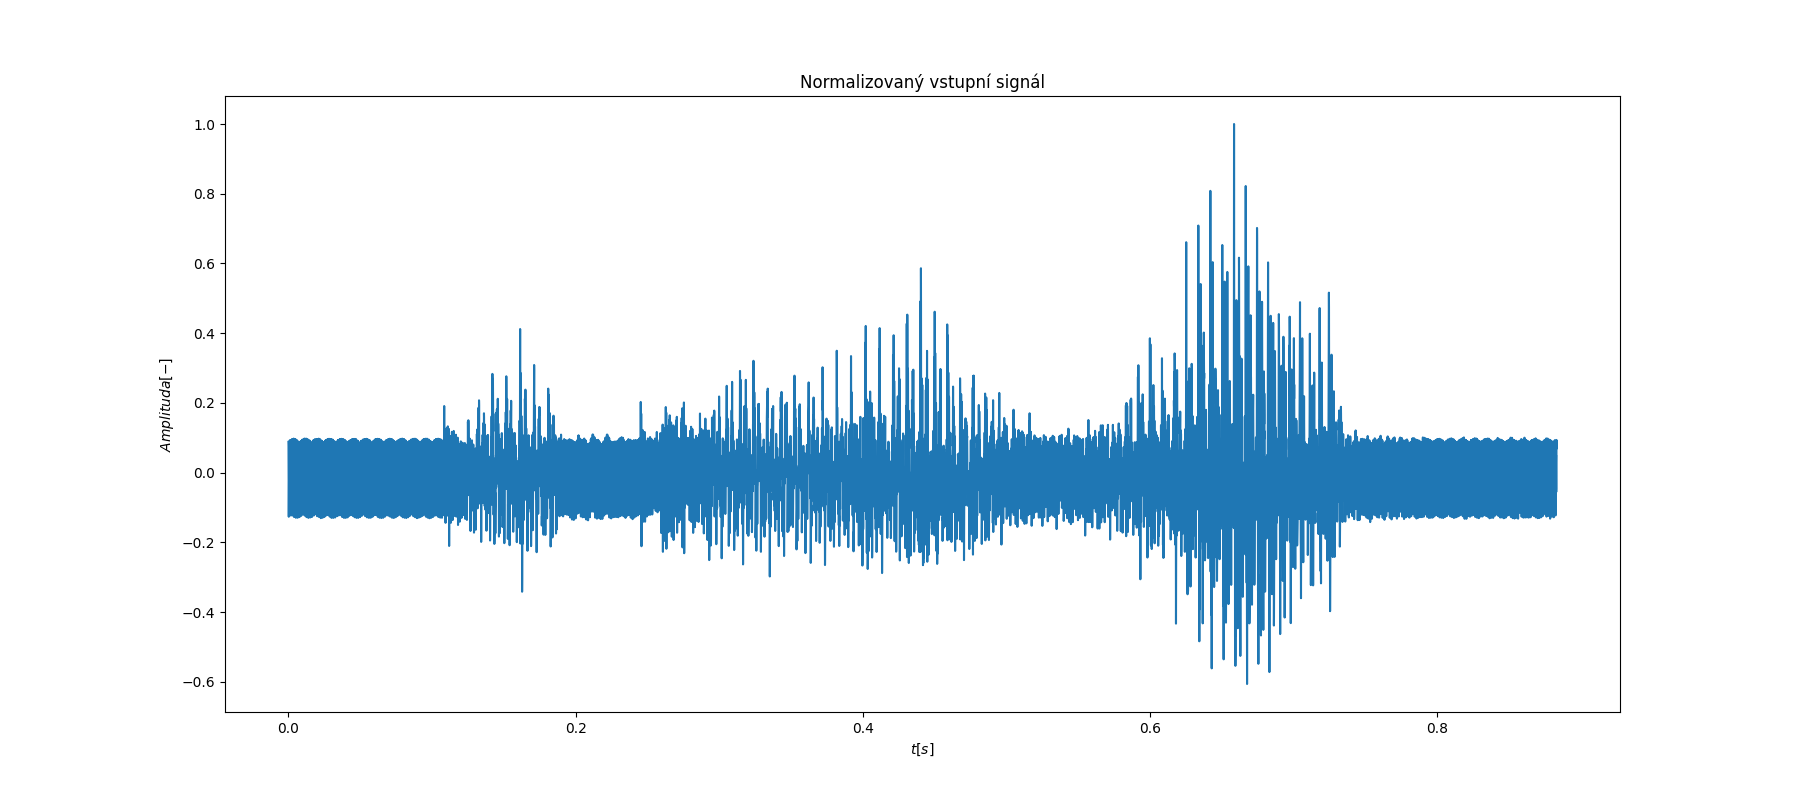
\includegraphics[scale=0.35,keepaspectratio]{Figure_3}
	\caption{Normalizovaný a vycentrovaný vstupní signál}
\end{figure}

\begin{figure}[H] 
	\centering
	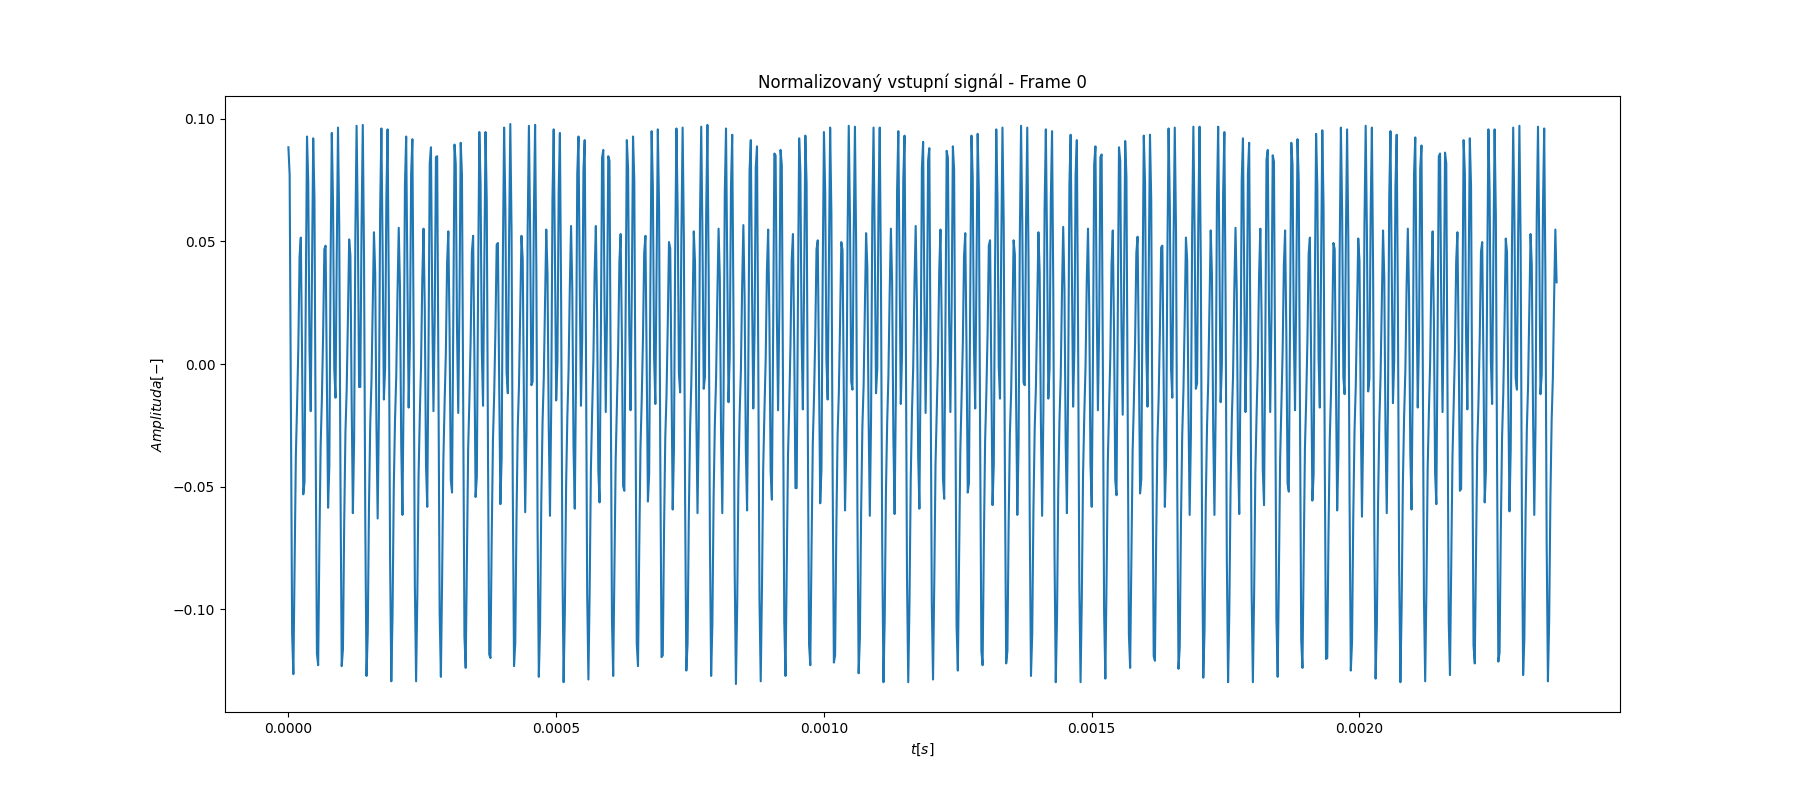
\includegraphics[scale=0.35,keepaspectratio]{Figure_2}
	\caption{Vycentrovaný a normalizovaný rámec \#0}
\end{figure}

\section{DFT}

Z grafů (i kódu) je patrné že výstup naší a vestavěné fouriérovy transformace jsou hodně podobné, takže naši implementaci můžeme považovat za správnou.

\begin{landscape}
\begin{figure}[H]
	\centering
	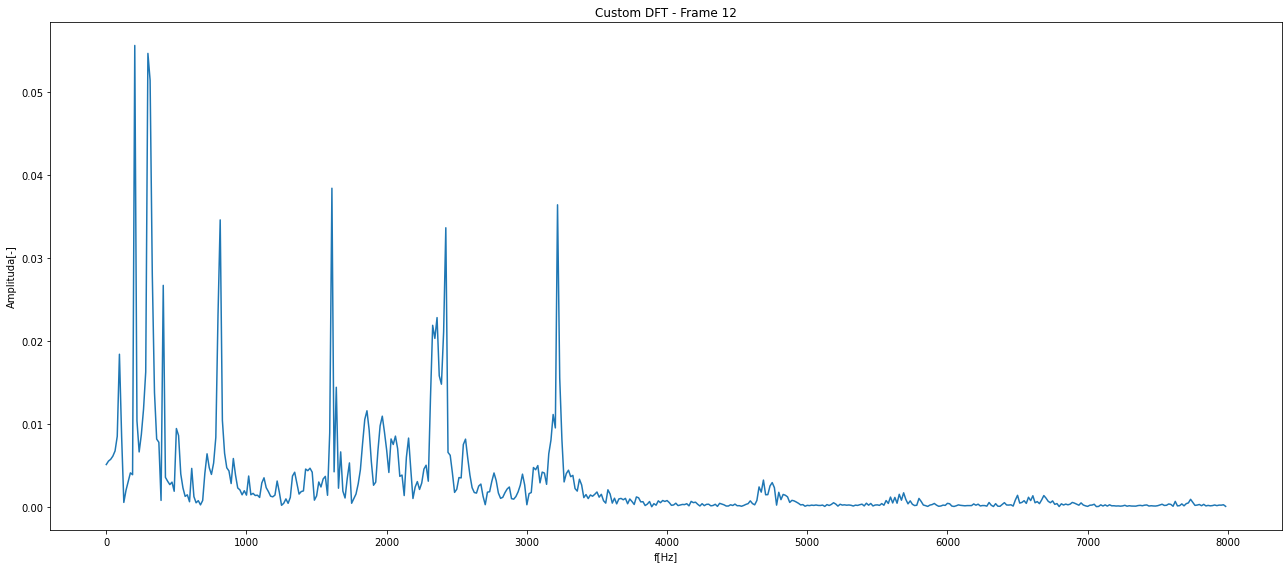
\includegraphics[scale=0.5,keepaspectratio]{Figure_5}
	\caption{Custom implementovaná funkce DFT}
\end{figure}
\end{landscape}

\begin{landscape}
\begin{figure}[H] 
	\centering
	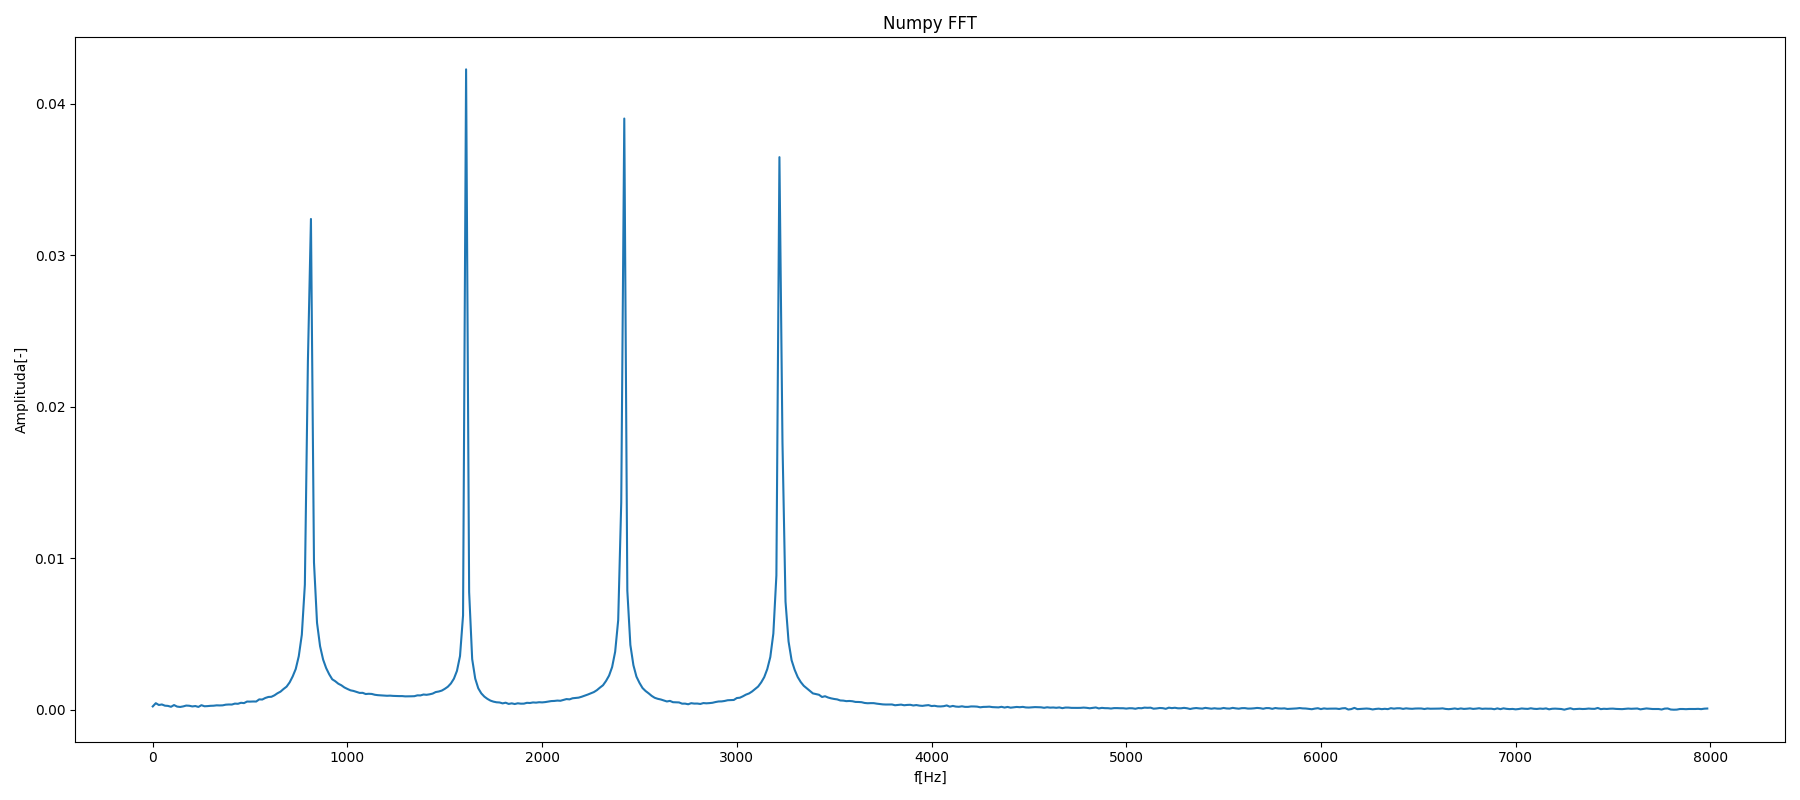
\includegraphics[scale=0.5,keepaspectratio]{Figure_4}
	\caption{Buildin FFT z knihovny numpy}
\end{figure}
\end{landscape}

\section{Spektrogram}
\begin{figure}[H] 
	\centering
	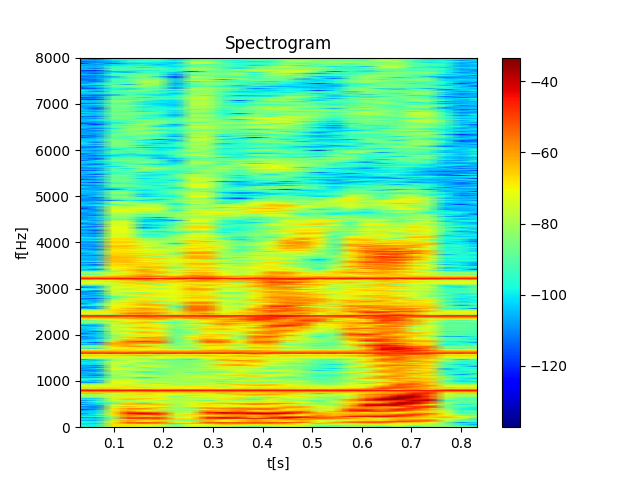
\includegraphics[scale=0.7,keepaspectratio]{Figure_6}
	\caption{Výkonový spektrogram}
\end{figure}

\begin{figure}[H] 
	\centering
	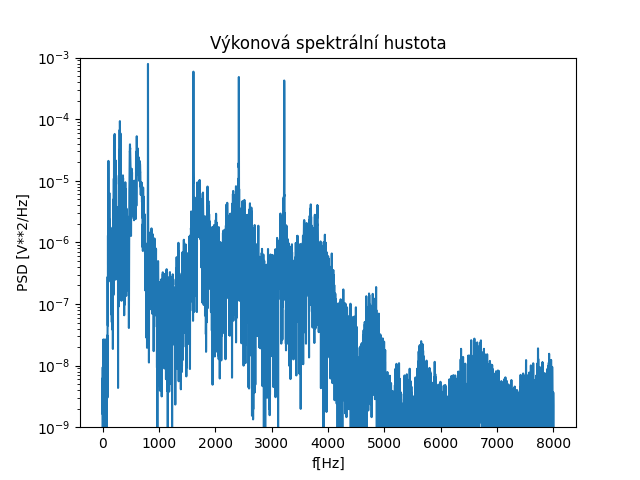
\includegraphics[scale=0.7,keepaspectratio]{Figure_7}
	\caption{Výkonová spektrální hustota}
\end{figure}

\begin{figure}[H] 
	\centering
	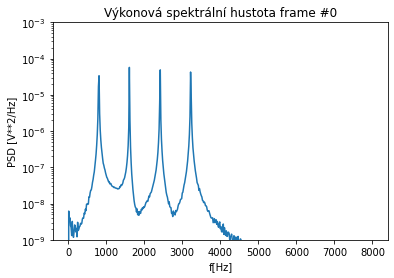
\includegraphics[scale=0.7,keepaspectratio]{Figure_26}
	\caption{Výkonová spektrální hustota frame \#0}
\end{figure}

\section{Určení rušivých frekvencí}
Z grafů výše můžeme vidět, že peaky rušení jsou +- stejně daleko od sebe, takže můžeme říci že jsou harmonicky vztažené neboli, že frekvence rušení 2., 3., 4., jsou násobky 1.
Z FFT grafu z úlohy 3 můžeme odečíst hodnoty frekvencí peaků, které jsou 3223, 2423, 1615 a 800 Hz.
Dále byla naprogramována funkce na získání frekvencí rušení z výkonové spektrální hustoty.
Funkce vrátila hodnoty 307.954, 215.115, 606.85 a 486.838 Hz.
Tyto hodnoty se velmi blíží těm co byli odečteny z grafu, takže funkce funguje správně.

\section{Generování signálu}
Byl vygenerován zvukový soubor obsahující pouze rušení složený z cosinusovek frekvencí, které jsme našli. Tento signál byl poté podroben spektrální analýze.
Z výskedků této analýzy můžeme viděť, že náš odhad byl správný a frekvence +- odpovídají. Je zde ale odchylka +- 300Hz (hlavně u vyšších frekvencí). Přesně se nepovedlo určit její zdroj, jelikož jako vstupní signál beru přímo signál generovaný funkcí z cosinů a ne čtený ze souboru.

\begin{figure}[H] 
	\centering
	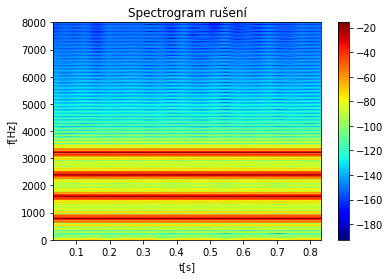
\includegraphics[scale=0.67,keepaspectratio]{Figure_8}
	\caption{Výkonový spektrogram rušení}
\end{figure}

\begin{figure}[H] 
	\centering
	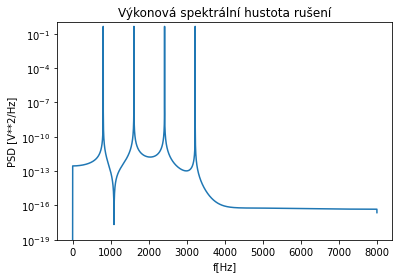
\includegraphics[scale=0.67,keepaspectratio]{Figure_9}
	\caption{Výkonová spektrální hustota rušení}
\end{figure}

\begin{landscape}
\begin{figure}[H] 
	\centering
	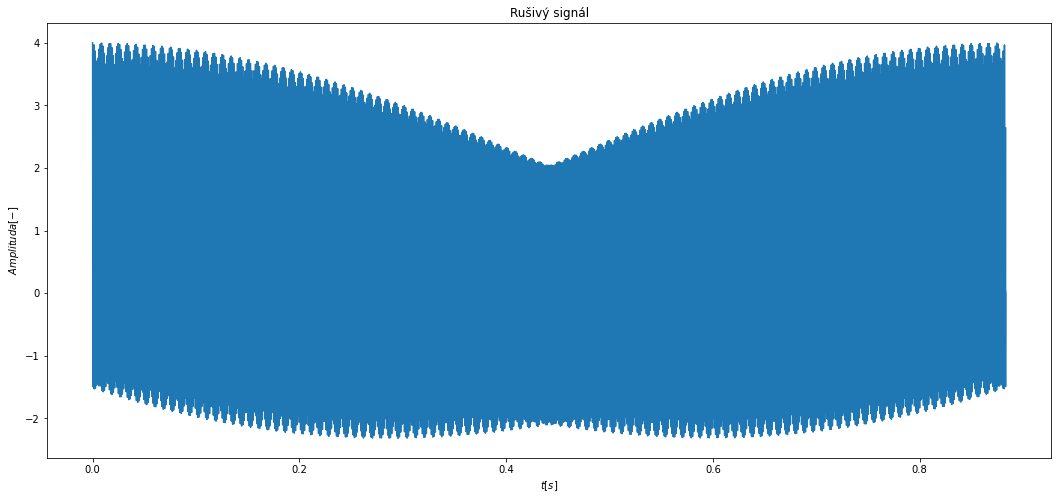
\includegraphics[scale=0.55,keepaspectratio]{Figure_25}
	\caption{Signál rušení}
\end{figure}
\end{landscape}

Můžeme vidět že signál nevypadá úplně přesně jako ve vstupním signálu a je to tím, že neznáme jeho amplitudu a počáteční fázy.


\section{Čistící filtr}

Byli navrženy 2 sady 4 filtrů typu pásmová zádrž na zablokování rušivých frekvencí (1 pro každou frekvenci).
Z grafů lze vidět, že Butterworthův filtr se po jednotkovém skoku nejrychleji ustálí na 0.

\begin{figure}[H] 
	\centering
	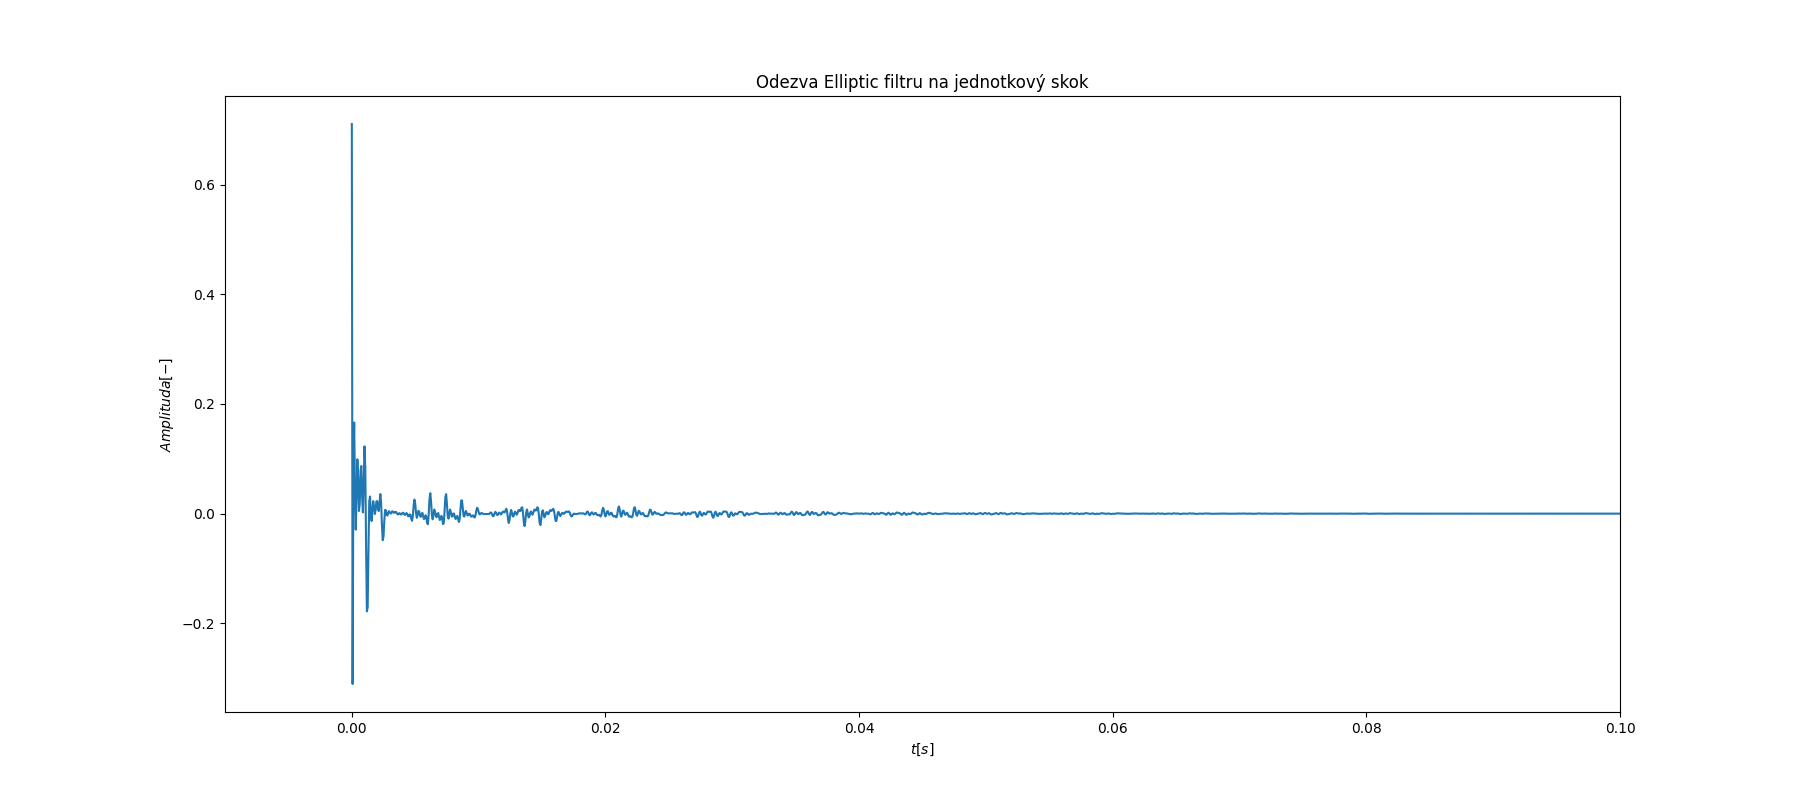
\includegraphics[scale=0.40,keepaspectratio]{Figure_22}
	\caption{Odezva na jednotkový skok Elliptic filtru}
\end{figure}

\begin{figure}[H] 
	\centering
	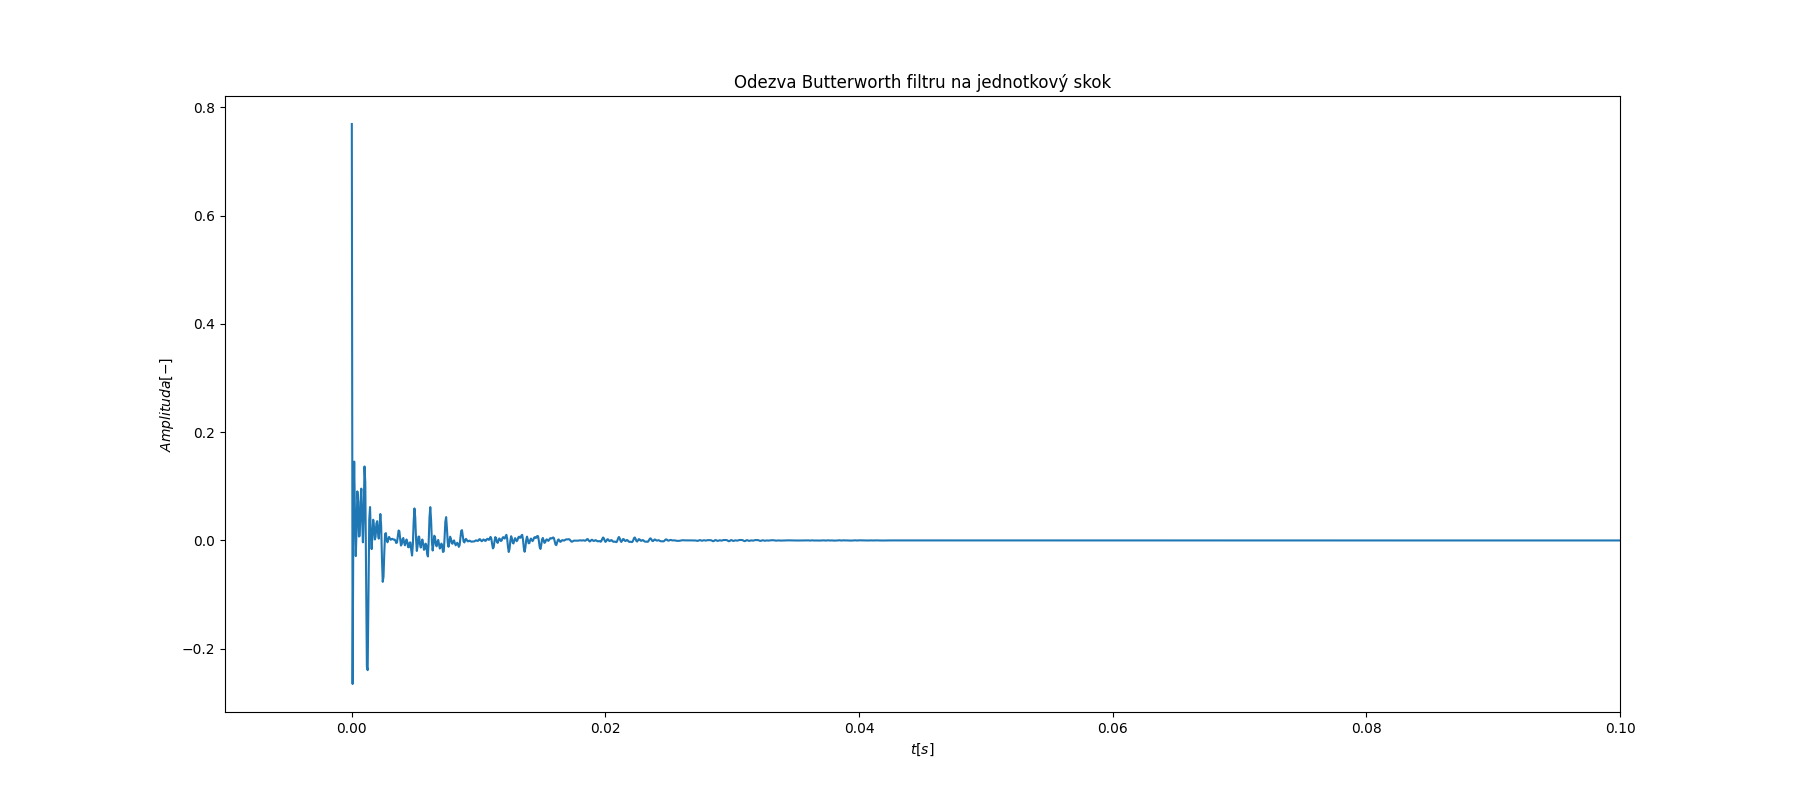
\includegraphics[scale=0.40,keepaspectratio]{Figure_24}
	\caption{Odezva na jednotkový skok Butterworth filtru}
\end{figure}

\section{Nulové body a póly}
\begin{figure}[H] 
	\centering
	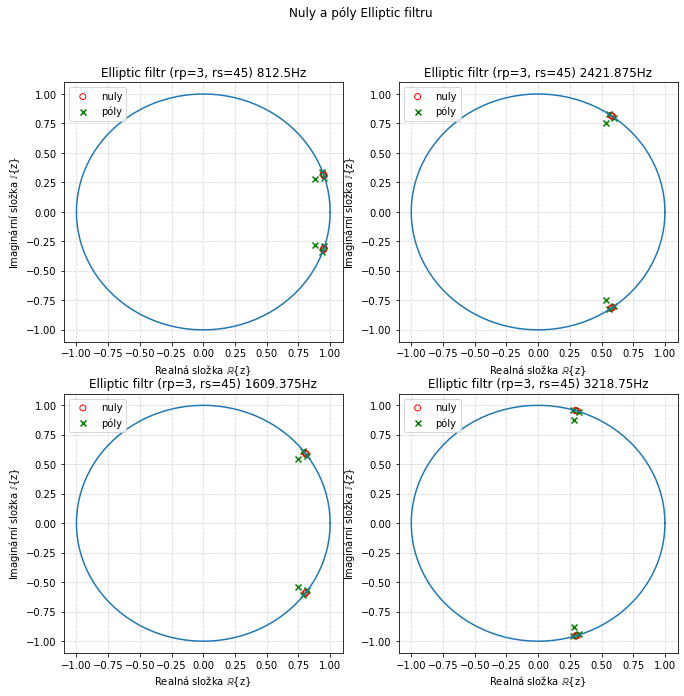
\includegraphics[scale=0.65,keepaspectratio]{Figure_19}
	\caption{Nulové body a póly Elliptic filtrů}
\end{figure}

\begin{figure}[H] 
	\centering
	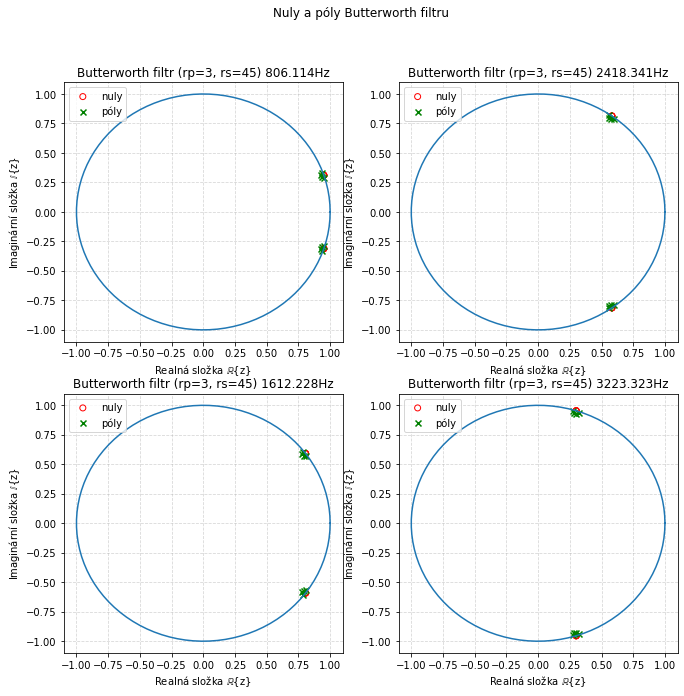
\includegraphics[scale=0.65,keepaspectratio]{Figure_18}
	\caption{Nulové body a póly Butterworthových filtrů}
\end{figure}

\newpage
\section{Frekvenční charakteristika}

Odečtením hodnot z grafu vycházejí očekávané frekvence, které jsme určili z spektrogramu, takže nastavení filtrů je dostatečné.
Následné další úpravy budou možné po aplikování filtrů na vstupní signál.

\subsection{Elliptic filtry}
\begin{figure}[H] 
	\centering
	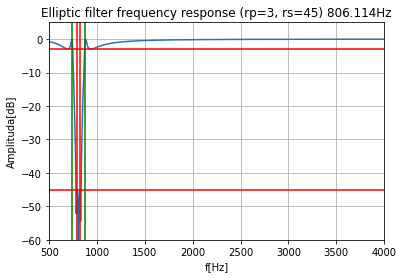
\includegraphics[scale=0.65,keepaspectratio]{Figure_10}
	\caption{Frekvenční charakteristika Elliptic filtru 1}
\end{figure}

\begin{figure}[H] 
	\centering
	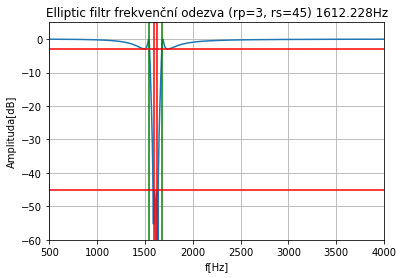
\includegraphics[scale=0.65,keepaspectratio]{Figure_11}
	\caption{Frekvenční charakteristika Elliptic filtru 2}
\end{figure}

\begin{figure}[H] 
	\centering
	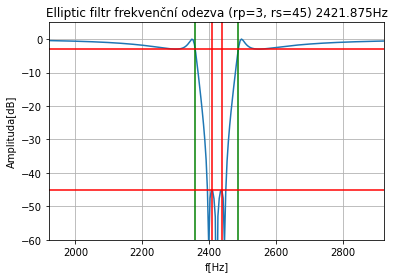
\includegraphics[scale=0.65,keepaspectratio]{Figure_12}
	\caption{Frekvenční charakteristika Elliptic filtru 3}
\end{figure}

\begin{figure}[H] 
	\centering
	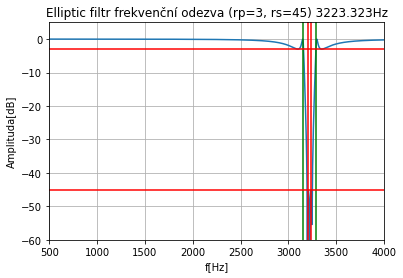
\includegraphics[scale=0.65,keepaspectratio]{Figure_13}
	\caption{Frekvenční charakteristika Elliptic filtru 4}
\end{figure}

\subsection{Butterworth filtry}
\begin{figure}[H] 
	\centering
	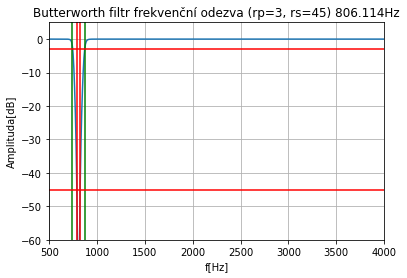
\includegraphics[scale=0.65,keepaspectratio]{Figure_14}
	\caption{Frekvenční charakteristika Butterworth filtru 1}
\end{figure}

\begin{figure}[H] 
	\centering
	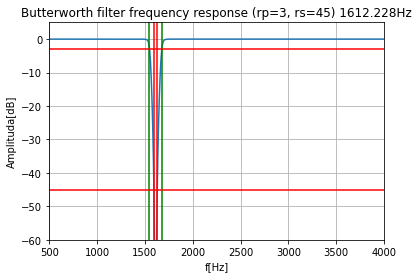
\includegraphics[scale=0.65,keepaspectratio]{Figure_15}
	\caption{Frekvenční charakteristika Butterworth filtru 2}
\end{figure}

\begin{figure}[H] 
	\centering
	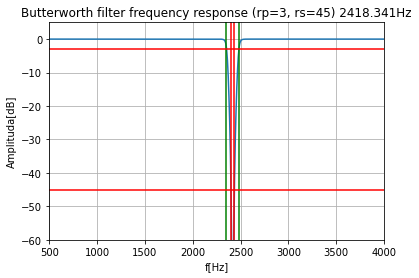
\includegraphics[scale=0.65,keepaspectratio]{Figure_16}
	\caption{Frekvenční charakteristika Butterworth filtru 3}
\end{figure}

\begin{figure}[H] 
	\centering
	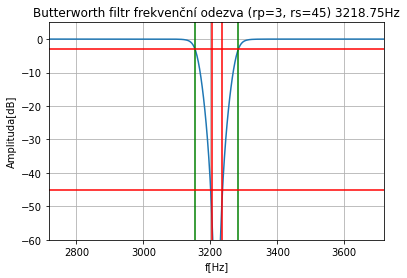
\includegraphics[scale=0.65,keepaspectratio]{Figure_17}
	\caption{Frekvenční charakteristika Butterworth filtru 4}
\end{figure}

\section{Filtrace}
\subsection{Elliptic filtry}
\begin{figure}[H] 
	\centering
	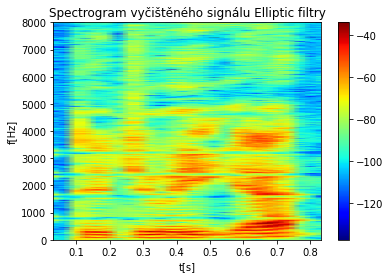
\includegraphics[scale=0.65,keepaspectratio]{Figure_20}
	\caption{Výkonový spektrogram vyčištěného signálu Elliptic filtry}
\end{figure}

\begin{figure}[H] 
	\centering
	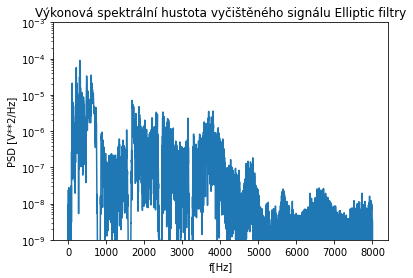
\includegraphics[scale=0.65,keepaspectratio]{Figure_21}
	\caption{Výkonová spektrální hustota vyčištěného signálu Elliptic filtry}
\end{figure}

\begin{landscape}
\begin{figure}[H] 
	\centering
	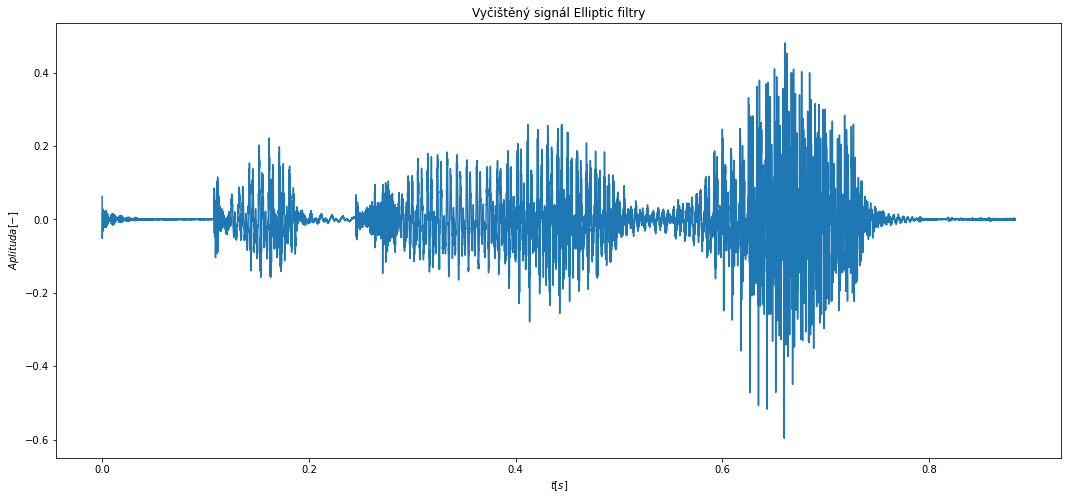
\includegraphics[scale=0.55,keepaspectratio]{Figure_23}
	\caption{Výsledný vyčištěný signál Elliptic filtry}
\end{figure}
\end{landscape}

\subsection{Butterworth filtry}
\begin{figure}[H] 
	\centering
	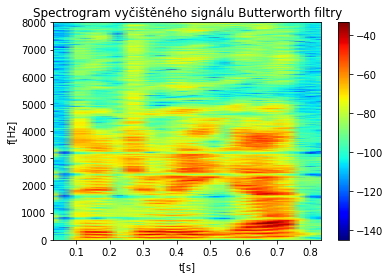
\includegraphics[scale=0.65,keepaspectratio]{Figure_27}
	\caption{Výkonový spektrogram vyčištěného signálu Butterworth filtry}
\end{figure}

\begin{figure}[H] 
	\centering
	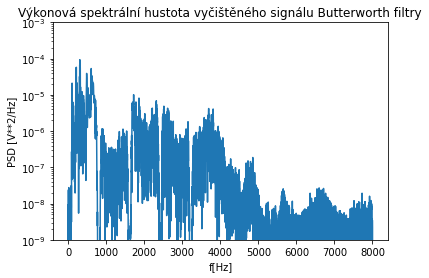
\includegraphics[scale=0.65,keepaspectratio]{Figure_28}
	\caption{Výkonová spektrální hustota vyčištěného signálu Butterworth filtry}
\end{figure}

\begin{landscape}
\begin{figure}[H] 
	\centering
	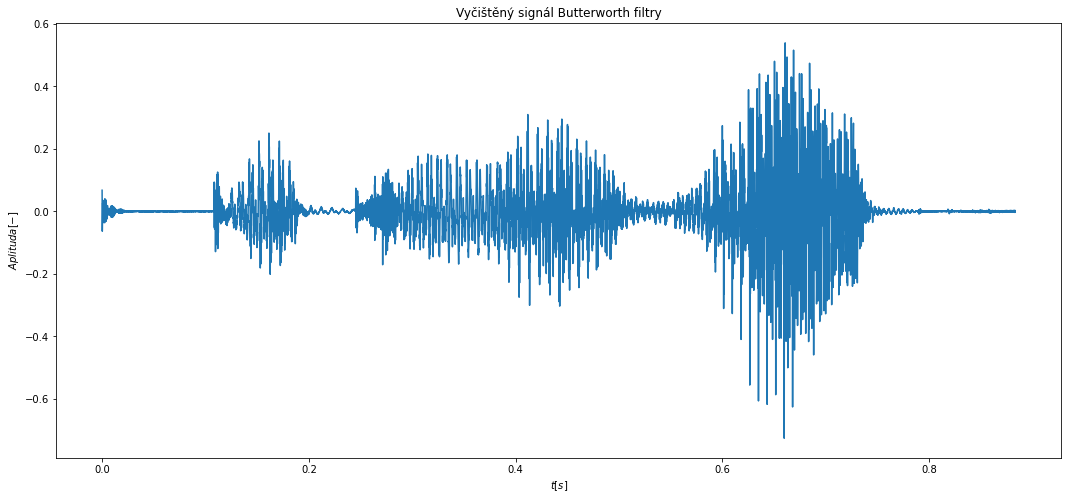
\includegraphics[scale=0.55,keepaspectratio]{Figure_29}
	\caption{Výsledný vyčištěný signál Butterworth filtry}
\end{figure}
\end{landscape}

\subsection{Shrnutí filtrace}
Vzhledem k tomu že se Butterworthův i Elliptic filtr chovali téměř identicky nebylo potřeba provádět čištění oběma.
Na výsledné číštění byl ale nakonec použit Elliptic filtr protože méně zkresluje signál na začátku a na konci.\\
Na spectrogramu vyčištěného signálu již nevidíme tak výrázné rušení i když nějaké rušení zde stále zůstalo. To může být způsobeno povahou rušení a nebo chováním filtru kde nemá na začátku ještě dostatek vzorků pro analýzu.
Můžeme vidět že i samotný signál je trochu zdeformovaný, což se dalo očekávat, jelikož část frekvenčního spektra tohoto signálu ležela ve stejné oblasti jako odstraňovaný šum.

\begin{landscape}
	\begin{figure}[H] 
		\centering
		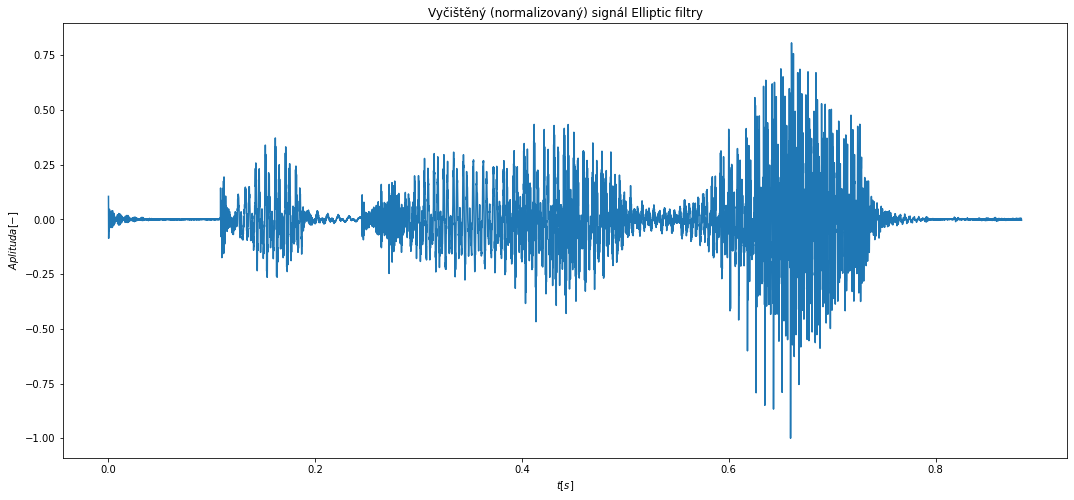
\includegraphics[scale=0.55,keepaspectratio]{Figure_30}
		\caption{Finální vyčištěný signál}
	\end{figure}
\end{landscape}

\end{document}